\documentclass[a4paper]{ctexart}
\usepackage[utf8]{inputenc}
\usepackage[a4paper]{geometry}
\usepackage{graphicx}
\usepackage{float}
\usepackage{hyperref}
\usepackage[heading = false]{ctex}
\usepackage{xcolor}
\usepackage{fontspec}
\usepackage{listings}
\usepackage{color}

\definecolor{dkgreen}{rgb}{0,0.6,0}
\definecolor{gray}{rgb}{0.5,0.5,0.5}
\definecolor{mauve}{rgb}{0.58,0,0.82}

\lstset{
  frame=tb,
  aboveskip=3mm,
  belowskip=3mm,
  showstringspaces=false,
  columns=flexible,
  basicstyle = \ttfamily,
  numbers=none,
  numberstyle=\tiny\color{gray},
  keywordstyle=\color{blue},
  commentstyle=\color{dkgreen},
  stringstyle=\color{mauve},
  breaklines=true,
  breakatwhitespace=true,
  tabsize=3
}
\pagestyle{plain}
\geometry{top=1.0cm, bottom=2.0cm}

\begin{document}
  \begin{titlepage}
      \songti
      \begin{center}
        \vspace*{2cm}
        
\includegraphics[width=0.7\textwidth]{../HDU.png}\\
        \vspace*{1cm}
        {\fontsize{36pt}{0}
          \textbf{机器学习实验\\报\quad 告\\}
        }
        \vspace*{12cm}
        {\fontsize{18pt}{0}
          \makebox[80pt]{\textbf{实验名称}} \underline{\makebox[250pt]{\Large 无监督学习之聚类}}\\
          \vspace*{0.5cm}
          \makebox[80pt]{\textbf{学\qquad 院}} \underline{\makebox[250pt]{\Large 通信工程学院}}\\
          \vspace*{0.5cm}
          \makebox[80pt]{\textbf{专\qquad 业}} \underline{\makebox[250pt]{\Large xxxx}}\\
          \vspace*{0.5cm}
          \makebox[80pt]{\textbf{学\qquad 号}} \underline{\makebox[250pt]{\Large xxxx}}\\
          \vspace*{0.5cm}
          \makebox[80pt]{\textbf{学生姓名}} \underline{\makebox[250pt]{\Large xxx}}\\
        }
      \end{center}
  \end{titlepage}

  \CTEXsetup[format={\Large\bfseries}]{section}

  \newpage
  \section{实验目的}
  \begin{enumerate}
    \item 理解无监督学习中各聚类算法原理
    \item 掌握Sklearn实现基于K-means方法及应用
  \end{enumerate}

  \section{实验内容与要求}
  \textbf{K-means聚类算法}

  \begin{itemize}
    \item K-means算法以k为参数,把n个对象分成k个簇,使簇内具有较高的相似度,而簇间的相似度较低
    \item 其处理过程如下
    \begin{enumerate}
      \item 随机选择k个点作为初始的聚类中心
      \item 对于剩下的点,根据其与聚类中心的距离,将其归入最近的簇
      \item 对每个簇,计算所有点的均值作为新的聚类中心
      \item 重复2、3直到聚类中心不再发生改变
    \end{enumerate}
  \end{itemize}
  \textbf{数据介绍}
  \begin{itemize}
    \item 现有1999年全国31个省份城镇居民家庭平均每人全年消费性支出的八个主要变量数据,
    这八个变量分别是:食品、衣着、家庭设备用品及服务、医疗保健、交通和通讯、娱乐教育文化服务、
    居住以及杂项商品和服务。利用已有数据,对31个省份进行聚类
    \item 通过聚类,了解1999年国内各个省份的消费水平情况
  \end{itemize}

  \section{实验程序与结果}
  \subsection{程序代码}
  \lstinputlisting[language=Python]{lab6.py}
  \subsection{运行结果}
  \begin{figure}[H]
    \centering
    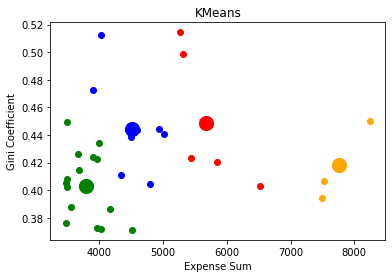
\includegraphics[width=0.7\textwidth]{fig/output.png}
    \caption{图中同一颜色的点为一类,较大的圆点为聚类中心}
  \end{figure}

  \section{实验结果分析}
  由于数据特征维度较高,因此对结果可视化时做了降维处理,X坐标表示总支出,
  Y坐标食品支出占总支出的比例,即基尼系数。

  从图中可以看出,K-Means将数据大致上分为了比较接近的4类,能够一定程度上反应消费水平。
  收入较低和较高的人群的基尼系数都较低,收入中等水平的人群基尼系数较高

  \section{实验问题解答与体会}
  本次实验使用了无监督学习的K-means方法,了解了无监督学习模型的特点,
  也对K-means的原理和效果有了更深的理解

\end{document}
